\documentclass[a4paper,11pt]{article}%,twocolumn
%\documentclass[a4paper,11pt]{article}
%% packages

\usepackage{blindtext} % needed for creating dummy text passages
%\usepackage{ngerman} % needed for German default language
\usepackage{amsmath} % needed for command eqref
\usepackage{amssymb} % needed for math fonts
\usepackage[colorlinks=true,breaklinks]{hyperref} % needed for creating hyperlinks in the document, the option colorlinks=true gets rid of the awful boxes, breaklinks breaks lonkg links (list of figures), and ngerman sets everything for german as default hyperlinks language
\usepackage[hyphenbreaks]{breakurl} % ben�tigt f�r das Brechen von URLs in Literaturreferenzen, hyphenbreaks auch bei links, die �ber eine Seite gehen (mit hyphenation).
\usepackage{xcolor}
\definecolor{c1}{rgb}{0,0,1} % blue
\definecolor{c2}{rgb}{0,0.3,0.9} % light blue
\definecolor{c3}{rgb}{0.3,0,0.9} % red blue
\hypersetup{
    linkcolor={c1}, % internal links
    citecolor={c2}, % citations
    urlcolor={c3} % external links/urls
}
%\usepackage{cite} % needed for cite
\usepackage[square,authoryear]{natbib} % needed for cite and abbrvnat bibliography style
\usepackage[nottoc]{tocbibind} % needed for displaying bibliography and other in the table of contents
\usepackage{graphicx} % needed for \includegraphics 
\usepackage{longtable} % needed for long tables over pages
\usepackage{bigstrut} % needed for the command \bigstrut
\usepackage{enumerate} % needed for some options in enumerate
%\usepackage{todonotes} % needed for todos
\usepackage{makeidx} % needed for creating an index
\makeindex
\usepackage{gensymb}
\usepackage{url}
\usepackage{psfrag}
\usepackage{multirow}
\usepackage{natbib}
\usepackage{pgf-pie}
\usepackage{tikz}
\usepackage{eso-pic}
\usepackage{subcaption}
\usepackage{cite}

%% page settings

\usepackage[top=20mm, bottom=20mm,left=20mm,right=20mm]{geometry} % needed for page border settings
\parindent=0mm % for space of first line of new text block
\sloppy % for writing with hyphenless justification (tries to)
\hyphenation{} % use hyphenation of tolerance parametershttp://www.jr-x.de/publikationen/latex/tipps/zeilenumbruch.html
\hyphenpenalty=10000
\exhyphenpenalty=10000
\usepackage{fancyhdr} % needed for head and foot options
%% my macros

%% Text fomats
\newcommand{\tbi}[1]{\textbf{\textit{#1}}}

%% Math fonts
\newcommand{\bbA}{\mathbb{A}}
\newcommand{\bbB}{\mathbb{B}}
\newcommand{\bbC}{\mathbb{C}}
\newcommand{\bbD}{\mathbb{D}}
\newcommand{\bbE}{\mathbb{E}}
\newcommand{\bbF}{\mathbb{F}}
\newcommand{\bbG}{\mathbb{G}}
\newcommand{\bbH}{\mathbb{H}}
\newcommand{\bbI}{\mathbb{I}}
\newcommand{\bbJ}{\mathbb{J}}
\newcommand{\bbK}{\mathbb{K}}
\newcommand{\bbL}{\mathbb{L}}
\newcommand{\bbM}{\mathbb{M}}
\newcommand{\bbN}{\mathbb{N}}
\newcommand{\bbO}{\mathbb{O}}
\newcommand{\bbP}{\mathbb{P}}
\newcommand{\bbQ}{\mathbb{Q}}
\newcommand{\bbR}{\mathbb{R}}
\newcommand{\bbS}{\mathbb{S}}
\newcommand{\bbT}{\mathbb{T}}
\newcommand{\bbU}{\mathbb{U}}
\newcommand{\bbV}{\mathbb{V}}
\newcommand{\bbW}{\mathbb{W}}
\newcommand{\bbX}{\mathbb{X}}
\newcommand{\bbY}{\mathbb{Y}}
\newcommand{\bbZ}{\mathbb{Z}}


\begin{document}
	
\begin{titlepage}
\center % Center everything on the page

%-------------------------------------------------------------------------------------
%	HEADING SECTIONS
%------------------------------------------------------------------------------------
\textbf{\large Department of Electronic and Telecommunication Engineering}\\[0.5cm]
\textbf{\Large University of Moratuwa, Sri Lanka}\\[1cm]
\textbf{\large EN 1190 - Engineering Design Project}\\[2cm]

\includegraphics[width=0.3\textwidth]{figures/uomlogo}\\[2cm]


	
%-------------------------------------------------------------------------------------
%	TITLE SECTION
%------------------------------------------------------------------------------------
\textbf{\Huge TrailGuard\\[1cm]by \\[0.5cm] Electrosquad}\\[2cm]
%\textbf{\Large A comparison}\\[7cm]


%----------------------------------------------------------------------------------------
%	MEMBERS SECTION
%----------------------------------------------------------------------------------------

\textbf{\large }\\[0.5cm]
{\large Balasooriya B A P I} \hspace{1.3cm}{\large 220054N  }\\
{\large Dewasumithra M P O} \hspace{1cm}{\large 220112R  }\\
{\large Dineshara M C} \hspace{2.3cm}{\large 220128V  }\\
{\large Diunugala C H} \hspace{2.3cm}{\large 220143L}\\[1cm]

%----------------------------------------------------------------------------------------
%	DATE SECTION
%----------------------------------------------------------------------------------------
\textbf{\large}\\[0.5cm]
\textbf{\Large \today} % Date, change the \today to a set date if you want to be precise

%----------------------------------------------------------------------------------------

\vfill % Fill the rest of the page with whitespace

\end{titlepage}
\newpage
\thispagestyle{empty}

\begin{tikzpicture}[remember picture, overlay]
\node[anchor=center] at (current page.center) {
    
\includegraphics[width=0.5\textwidth]{figures/TrailGuardLogo.png}
};
\end{tikzpicture}
\newpage
\tableofcontents
\pagebreak

% figures/TrailGuardLogo.png
%------------------------------------------------------------------------

\section{Problem Description}


%----------------------------------------------------------------------

\subsection{Problem}
In today’s rapidly changing environment, outdoor enthusiasts such as hikers, cavers, and travelers face increasing challenges related to environmental conditions. The quality of air and water is not always visible, yet it plays a crucial role in health and safety. Hikers often encounter water sources during their journeys, but determining whether the water is safe for drinking or swimming is difficult without proper equipment. Additionally, exposure to harmful gases, especially in caves or enclosed spaces, can be hazardous. The lack of portable, comprehensive solutions that monitor these vital environmental parameters poses a significant risk to those who venture into nature.

\subsection{Solution}
TrailGuard is a portable device designed to address these challenges by providing real-time monitoring of key environmental parameters such as air quality, water quality, temperature, and humidity. Equipped with a range of sensors, including a TS-300B turbidity sensor, PH4502C pH sensor, DHT11 temperature and humidity sensor, Sharp GP2Y1010AU0F dust sensor, and MQ2 gas sensor, TrailGuard offers a comprehensive solution for assessing environmental conditions. The device also includes a buzzer and LED indicator to alert users to potential dangers, making it a valuable addition to any hiker's gear. The Atmega328P-AU microcontroller serves as the brain of the device, ensuring efficient operation and control over the various sensors and user interfaces.

\subsection{Motivation}
The motivation behind TrailGuard stems from the growing need for safety and awareness among outdoor enthusiasts. With the increasing popularity of hiking, caving, and other outdoor activities, there is a rising demand for reliable tools that can help individuals assess and respond to environmental risks. TrailGuard aims to empower users with the knowledge they need to make informed decisions about the air they breathe, the water they encounter, and the overall environmental conditions during their adventures. By providing a portable, user-friendly solution, TrailGuard enhances the safety and enjoyment of outdoor experiences.

\subsection{Justification}
The development of TrailGuard is justified by the clear demand for a compact, reliable device that addresses multiple environmental concerns in one package. 

To validate the problem and understand the needs and preferences of potential users, we conducted a survey among hikers, adventurers, and students across universities in Sri Lanka. Out of 150 responses, we randomly selected 100 samples for analysis.
\\ 
\\
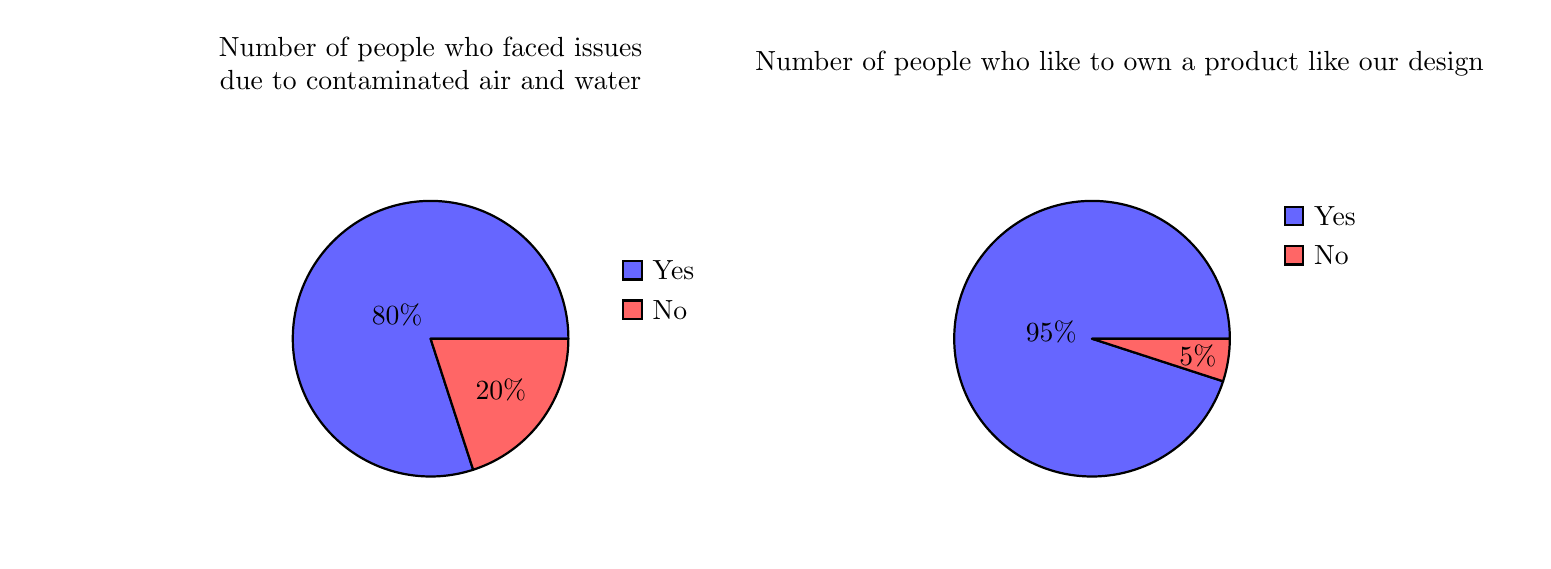
\begin{tikzpicture}[scale=0.7]
    % 2008 Pie Chart
	\node at (0,3.5) {};
	Tesr
    \pie[pos={0,0}, text=legend, radius=2.5, color={blue!60, red!60}, sum=100, after number=\%]{
        80/Yes,
        20/No
    }
    \node[text width=10cm, align=center] at (0,5) {Number of people who faced issues due to contaminated air and water};
    
    % 2009 Pie Chart
    \pie[pos={12,0}, text=legend, radius=2.5, color={blue!60, red!60}, sum=100, after number=\%]{
        95/Yes,
        5/No
    }
    \node at (15,-3.5) {};
	\node[text width=10cm, align=center] at (12.5,5) {Number of people who like to own a product like our design};
    
\end{tikzpicture}
\\
\\
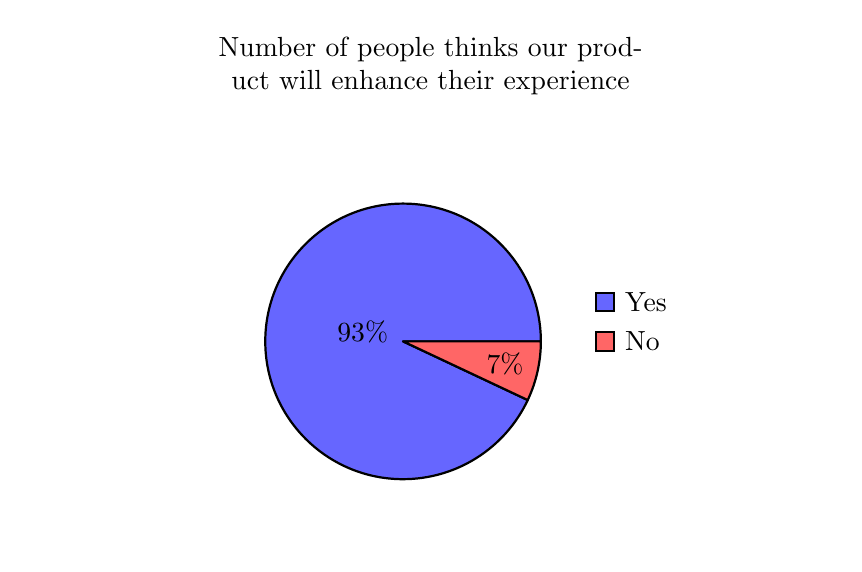
\begin{tikzpicture}[scale=0.7]    
    % 2010 Pie Chart
    \pie[pos={12,0}, text=legend, radius=2.5, color={blue!60, red!60}, sum=100, after number=\%]{
        93/Yes,
        7/No
    }
    \node at (12,-3.5) {};
	\node[text width=10cm, align=center] at (12.5,5) {Number of people thinks our product will enhance their experience};
\end{tikzpicture}

The survey revealed significant concerns about environmental safety during outdoor activities. Notably, 80\% of respondents reported facing issues due to contaminated air and water while traveling. Despite this, only one respondent owned a device capable of measuring water quality. 

The majority of participants (95\%) expressed a strong interest in owning a product like TrailGuard, and 93\% believed that such a device would enhance their overall travel experience.

Furthermore, our research indicated a lack of existing products that offer the same combination of functionalities as TrailGuard. While there are devices available that measure either water or air quality, they tend to be expensive and lack the comprehensive monitoring capabilities of our design. Additionally, social media research highlighted frequent complaints from tourists in the South Asian region about unknowingly drinking contaminated water, leading to unexpected health issues during their travels.

These factors, combined with the positive feedback from our survey, strongly support the need for TrailGuard. The device’s ability to monitor air and water quality, detect harmful gases, and measure temperature and humidity in a single, portable form factor makes it a valuable tool for enhancing safety and enjoyment during outdoor adventures.

\newpage
\section{Feasibility}
\subsection{Technical Feasibility}
The project technically feasible, and all resource requirements were met easily. 

We Designed the electronic circuits and designed the PCB in altium designer. The PCB was manufactured and assembled by a professional PCB manufacturer (JLC PCB). The software was developed using the Arduino IDE, and the final product was tested for functionality and performance.
We used Black PLA to 3D print the enclosure for the device. The device was assembled and tested for fit and functionality.
\subsubsection{Hardware Feasibility} 
The hardware components required for TrailGuard are readily available and well-suited for the device's intended functionality. The core of the system is the Atmega328P-AU microcontroller, a robust and reliable choice for managing multiple sensor inputs and controlling the device’s user interface. The selected sensors, including the TS-300B turbidity sensor, PH4502C pH sensor, DHT11 temperature and humidity sensor, Sharp GP2Y1010AU0F dust sensor, MQ2 gas sensor, and Gravity TDS sensor, are all compatible with the Atmega328P-AU and have been widely used in similar applications.
\\
\\
These sensors have been chosen for their accuracy, reliability, and low power consumption, which is critical for a portable device like TrailGuard. The device also incorporates an OLED display, buttons, a buzzer, and an LED indicator, all of which are easily integrated with the microcontroller. The hardware design also includes power-saving features, such as the ability to turn off the display and water sensors when not in use, which extends battery life. 
\subsubsection{Software Feasibility}
The software development for TrailGuard primarily involves programming the Atmega328P-AU microcontroller to manage the sensors, process the data, and control the user interface. The microcontroller can be programmed using the Arduino IDE, which is well-documented and widely supported, making it a practical choice for this project.
\\
\\
The software will need to handle real-time data acquisition from multiple sensors, perform basic data processing, and trigger alerts based on predefined thresholds for air and water quality. The user interface, controlled via the OLED display and buttons, will be designed to be intuitive and responsive, allowing users to easily access the information they need. The ability to switch off certain components to conserve power will also be managed through the software. 
\subsection{Economic Feasibility}
TrailGuard is designed to be an affordable solution for hikers, adventurers, and residents who are concerned about environmental safety. The components used in the device, such as the Atmega328P-AU microcontroller and various sensors, are cost-effective and widely available, which helps keep the overall production cost low.

By integrating multiple functionalities into a single device, TrailGuard offers significant value compared to purchasing separate devices for air and water quality monitoring, which tend to be more expensive. The cost of producing each unit is competitive, making it feasible to price the device at a level that is accessible to a broad range of customers. Additionally, the modular design and power-saving features contribute to a longer product lifespan, reducing the need for frequent replacements and further enhancing the device's economic appeal.






%--------------------------------------------------------------------------
\newpage
\section{Applications}
TrailGuard is a versatile device with a wide range of applications, particularly for outdoor enthusiasts, travelers, and individuals concerned about environmental safety. Below are the primary applications of TrailGuard
\subsection{Hiking and Outdoor Adventures}
One of the primary applications of TrailGuard is for hikers and outdoor adventurers. When exploring remote areas, access to clean water and fresh air can be unpredictable. TrailGuard helps users monitor the quality of water sources they encounter, ensuring that the water is safe for drinking or swimming. Additionally, the device can detect harmful gases and monitor air quality, alerting users to potential dangers, especially in enclosed spaces like caves. The portability and durability of TrailGuard make it an essential part of any hiker's gear, enhancing safety and providing peace of mind.

\subsection{Caving and Spelunking}
For cavers and spelunkers, air quality is a critical concern due to the potential presence of harmful gases in underground environments. TrailGuard’s gas detection capabilities, combined with its ability to measure temperature and humidity, make it an invaluable tool for those who explore caves. The device's compact design allows it to be easily carried and attached to gear, ensuring that it is always accessible when needed. The real-time alerts provided by TrailGuard can prevent accidents and health risks associated with poor air quality in these challenging environments.

\subsection{Environmental Monitoring for Residents}
TrailGuard is also valuable for residents in areas where environmental conditions may be a concern. Whether living near industrial zones, in areas with poor air quality, or regions prone to water contamination, residents can use TrailGuard to monitor their immediate environment. The device provides continuous feedback on air and water quality, allowing individuals to take proactive steps to protect their health. Its easy-to-use interface and portable design make it suitable for daily use around the home or in the community.

\subsection{Travel Safety}
Travelers often face uncertainties regarding the quality of air and water in unfamiliar regions. TrailGuard serves as a travel companion, providing crucial information about environmental conditions in real-time. This is particularly useful for tourists visiting regions where water quality may be compromised or where air pollution levels are high. By carrying TrailGuard, travelers can avoid potential health issues related to contaminated water or poor air quality, making their trips safer and more enjoyable.

\subsection{Educational and Research Purposes}
TrailGuard can also be utilized in educational settings and research projects focused on environmental science. Students and researchers can use the device to collect data on air and water quality in various environments. The portability and ease of use make it an excellent tool for field studies, allowing users to gather accurate and reliable data without the need for complex equipment. This application extends TrailGuard’s utility beyond personal safety, contributing to broader efforts in environmental monitoring and education.

%--------------------------------------------------------------------------
\newpage
\section{Product Architecture}
TrailGuard is designed with a modular architecture that integrates various hardware components and software systems to monitor environmental parameters efficiently. The architecture of TrailGuard can be broken down into the following key components

\subsection{Hardware Architecture}
The hardware architecture of TrailGuard is composed of several critical components that work together to collect, process, and display environmental data. The block diagram below illustrates the key hardware components and their interactions.
\begin{figure}[!h]
    \centering
    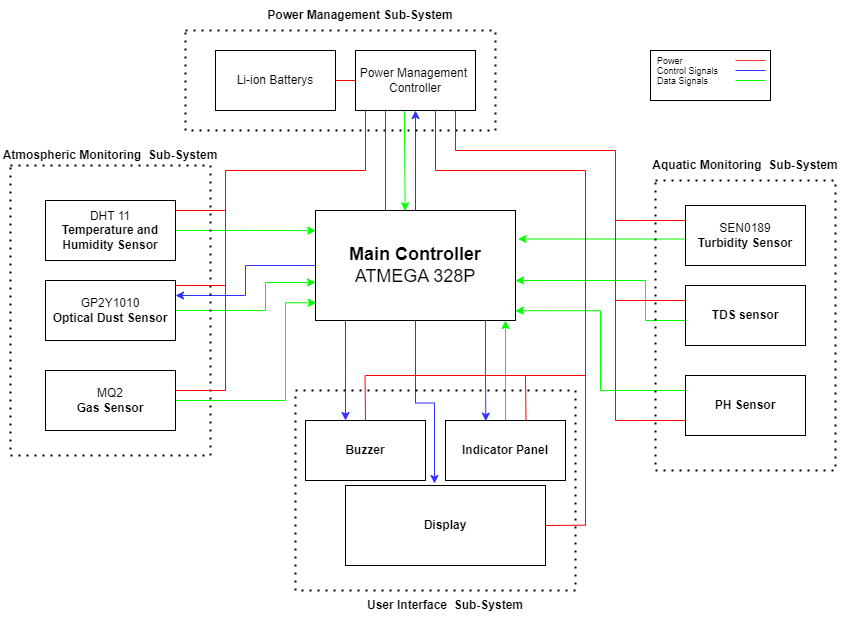
\includegraphics[scale=0.45]{figures/Block Diagram.png}
    \caption{Block Diagram of TrailGuard Hardware Architecture}
\end{figure}

\subsubsection{Microcontroller} 
The Atmega328P-AU microcontroller serves as the central processing unit of TrailGuard. It manages the operation of sensors, processes the data, and controls the output devices such as the OLED display, buzzer, and LED indicator.

\subsubsection{Sensors}


    \begin{tabular}{|p{0.3\textwidth}|p{0.7\textwidth}|}
    \hline
    \textbf{Sensor} & \textbf{Description} \\
    \hline
    TS-300B Turbidity Sensor & Measures the turbidity (cloudiness) of water to assess its quality. \\
    \hline
    PH4502C pH Sensor & Measures the pH level of water to determine its acidity or alkalinity. \\
    \hline
    DHT11 Temperature and Humidity Sensor & Monitors the ambient temperature and humidity levels. \\
    \hline
    Sharp GP2Y1010AU0F Dust Sensor & Detects the concentration of dust \& pollen particles in the air. \\
    \hline
    MQ2 Gas Sensor & Detects the presence of harmful gases such as carbon monoxide and smoke. \\
    \hline
    Gravity TDS Sensor & Measures the Total Dissolved Solids (TDS) in water, providing an indication of water purity. \\
    \hline
\end{tabular}



\subsubsection{Input/Output (IO) Devices}

    \begin{tabular}{|p{0.3\textwidth}|p{0.6\textwidth}|}
    \hline
    \textbf{I/O device} & \textbf{Description} \\
    \hline
    Buttons & Two buttons are used for navigating the user interface and controlling device functions. \\
    \hline
    Buzzer & Serves as an audible alert system, warning users of dangerous environmental conditions. \\
    \hline
    LED Indicator & Provides visual alerts, complementing the buzzer for immediate awareness. \\
    \hline
    OLED Display (0.96") & Provides a visual interface for users to view real-time sensor readings and alerts. It is compact, energy-efficient, and easy to read even in bright outdoor conditions. \\
    \hline
    \end{tabular}

\subsubsection{Power Management}

The MOSFET circuit allows selective power control, enabling the display and water sensors to be turned off when not in use to conserve battery life.
\subsubsection{Power Source} 
TrailGuard is powered by a 3200mAh 18650 Li-ion rechargeable battery, optimized for prolonged use during outdoor activities.

\subsection{Software Architecture}
The software architecture of TrailGuard is designed to be efficient, user-friendly, and responsive. 

\subsubsection{Firmware}
The microcontroller is programmed with firmware that handles sensor data acquisition, processing, and output control. The firmware is developed using the Arduino IDE and tools, taking advantage of its extensive library support and ease of use.

\subsubsection{Sensor Data Processing}
 The firmware continuously collects data from the connected sensors, processes it to filter noise, and compares it against predefined thresholds. If the data indicates a potential hazard (e.g., dangerous gas levels), the system triggers an alert through the buzzer and LED.
\\
\\
 Users can also measure each parameter individually by selecting the corresponding menu option on the display. The firmware ensures that the sensor readings are accurate and updated in real-time, providing users with reliable information about their environment.
 \subsubsection{User Interface}
 The OLED display and buttons create an interactive user interface, allowing users to view current sensor readings, navigate through menus, and configure device settings. The interface is designed to be intuitive, with clear visual cues and simple navigation.


 \subsubsection{Alert System}
 The software is programmed to trigger alerts based on specific environmental conditions. For example, the presence of harmful gases will activate the buzzer and LED indicator, ensuring users are immediately informed.


%------------------------------------------------------------------------
\section{Design and Product Enclosure}
\subsection{Design Overview}
The design of TrailGuard is centered around portability, durability, and user-friendliness. As a device intended for outdoor use, it is essential that TrailGuard is compact, lightweight, and robust enough to withstand the rigors of various environments, whether on a hiking trail, in a cave, or during travel. The design also focuses on integrating all necessary components in a way that maximizes functionality while minimizing size and weight.
\subsection{Enclosure Design} 
\begin{figure}[!h]
    \centering
    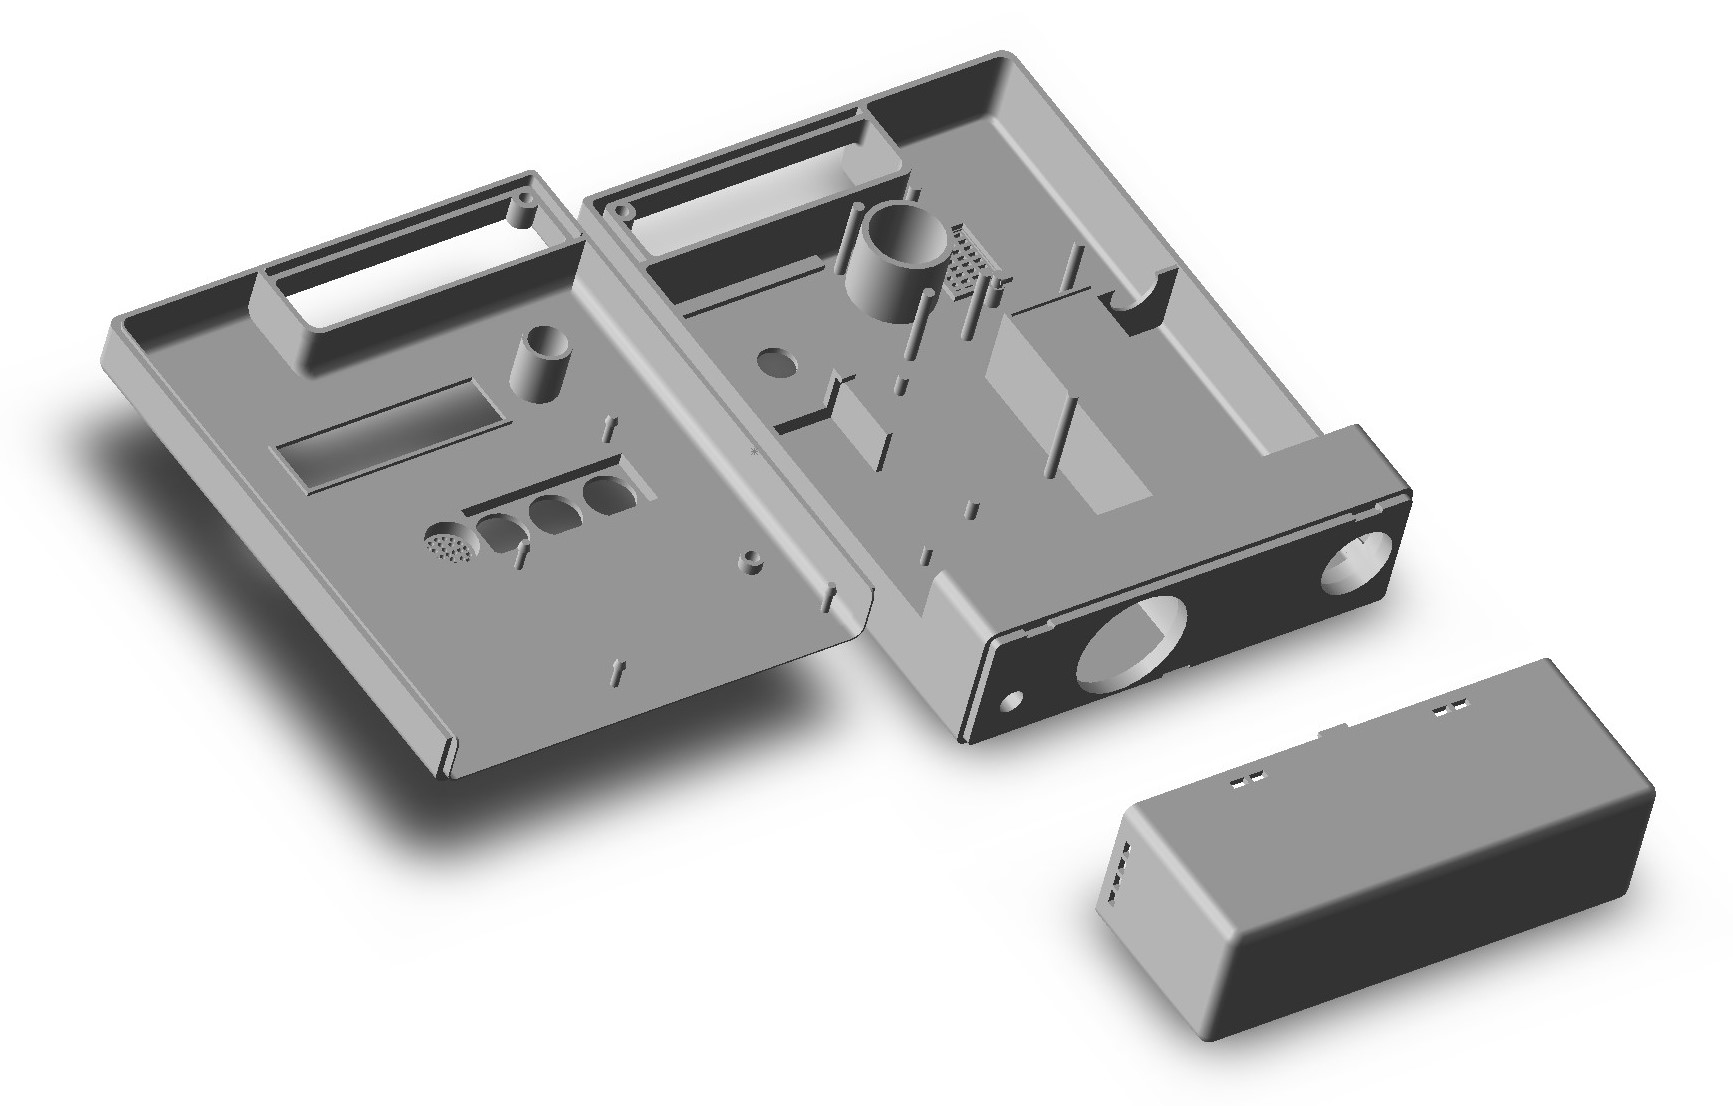
\includegraphics[scale=0.7]{figures/Enclosure.jpg}
    \caption{Block Diagram of TrailGuard Hardware Architecture}
\end{figure}
\subsection{Mounting and Portability}
To enhance portability, TrailGuard includes a built-in clip or loop that allows it to be securely attached to a backpack. This ensures that the device is always within reach and can be easily monitored without needing to be held or stored in a pocket. The attachment mechanism is designed to be sturdy, preventing accidental detachment during vigorous activities such as hiking or climbing.

%--------------------------------------------------------------------------
\newpage
\section{PCB}

\subsection{PCB Design}

\begin{figure}[!h]
    \centering
    \begin{subfigure}[b]{0.27\textwidth}
        \centering
        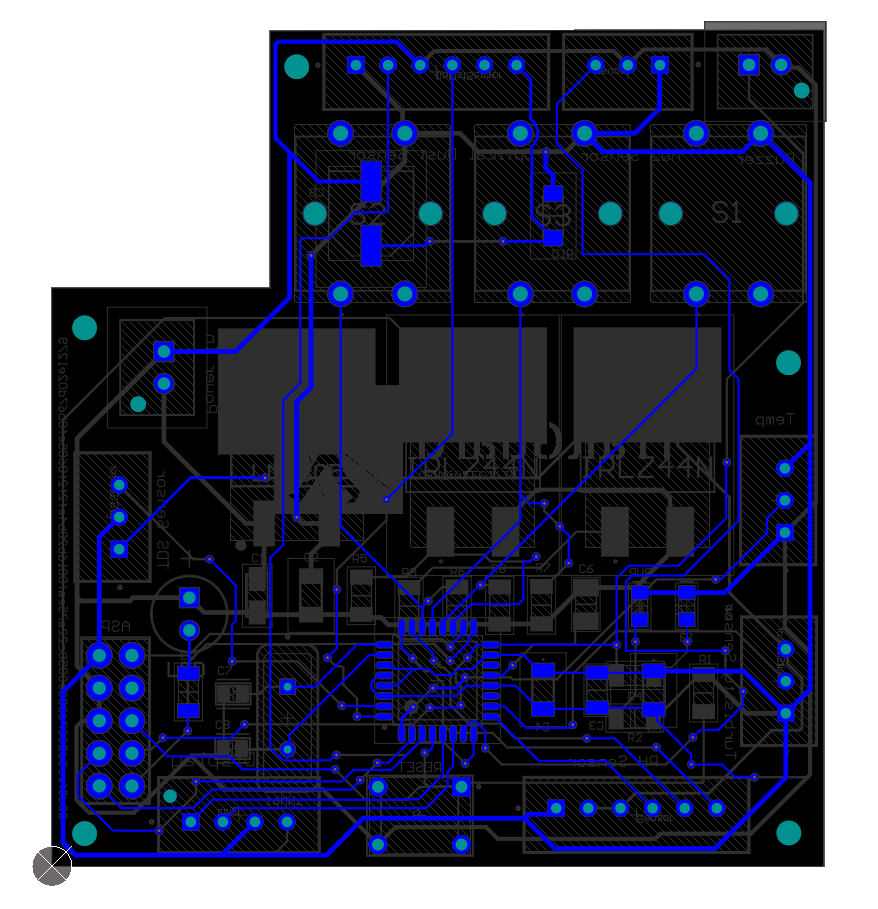
\includegraphics[width=\textwidth]{./figures/PCBBottomLayer.png}
        \caption{PCB Top Layer}
        \label{fig:image2}
    \end{subfigure}
    \hfill
    \begin{subfigure}[b]{0.27\textwidth}
        \centering
        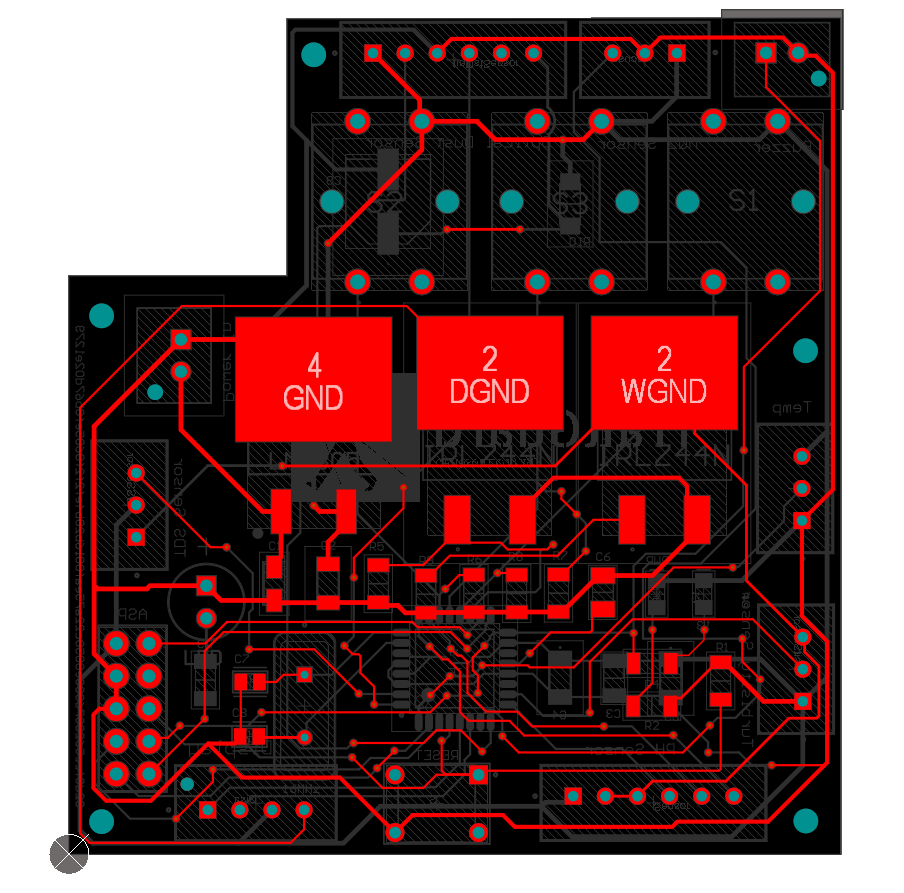
\includegraphics[width=\textwidth]{./figures/PCBTopLayer.png}
        \caption{PCB Bottom  Layer}
        \label{fig:image3}
    \end{subfigure}
    \begin{subfigure}[b]{0.36\textwidth}
        \centering
        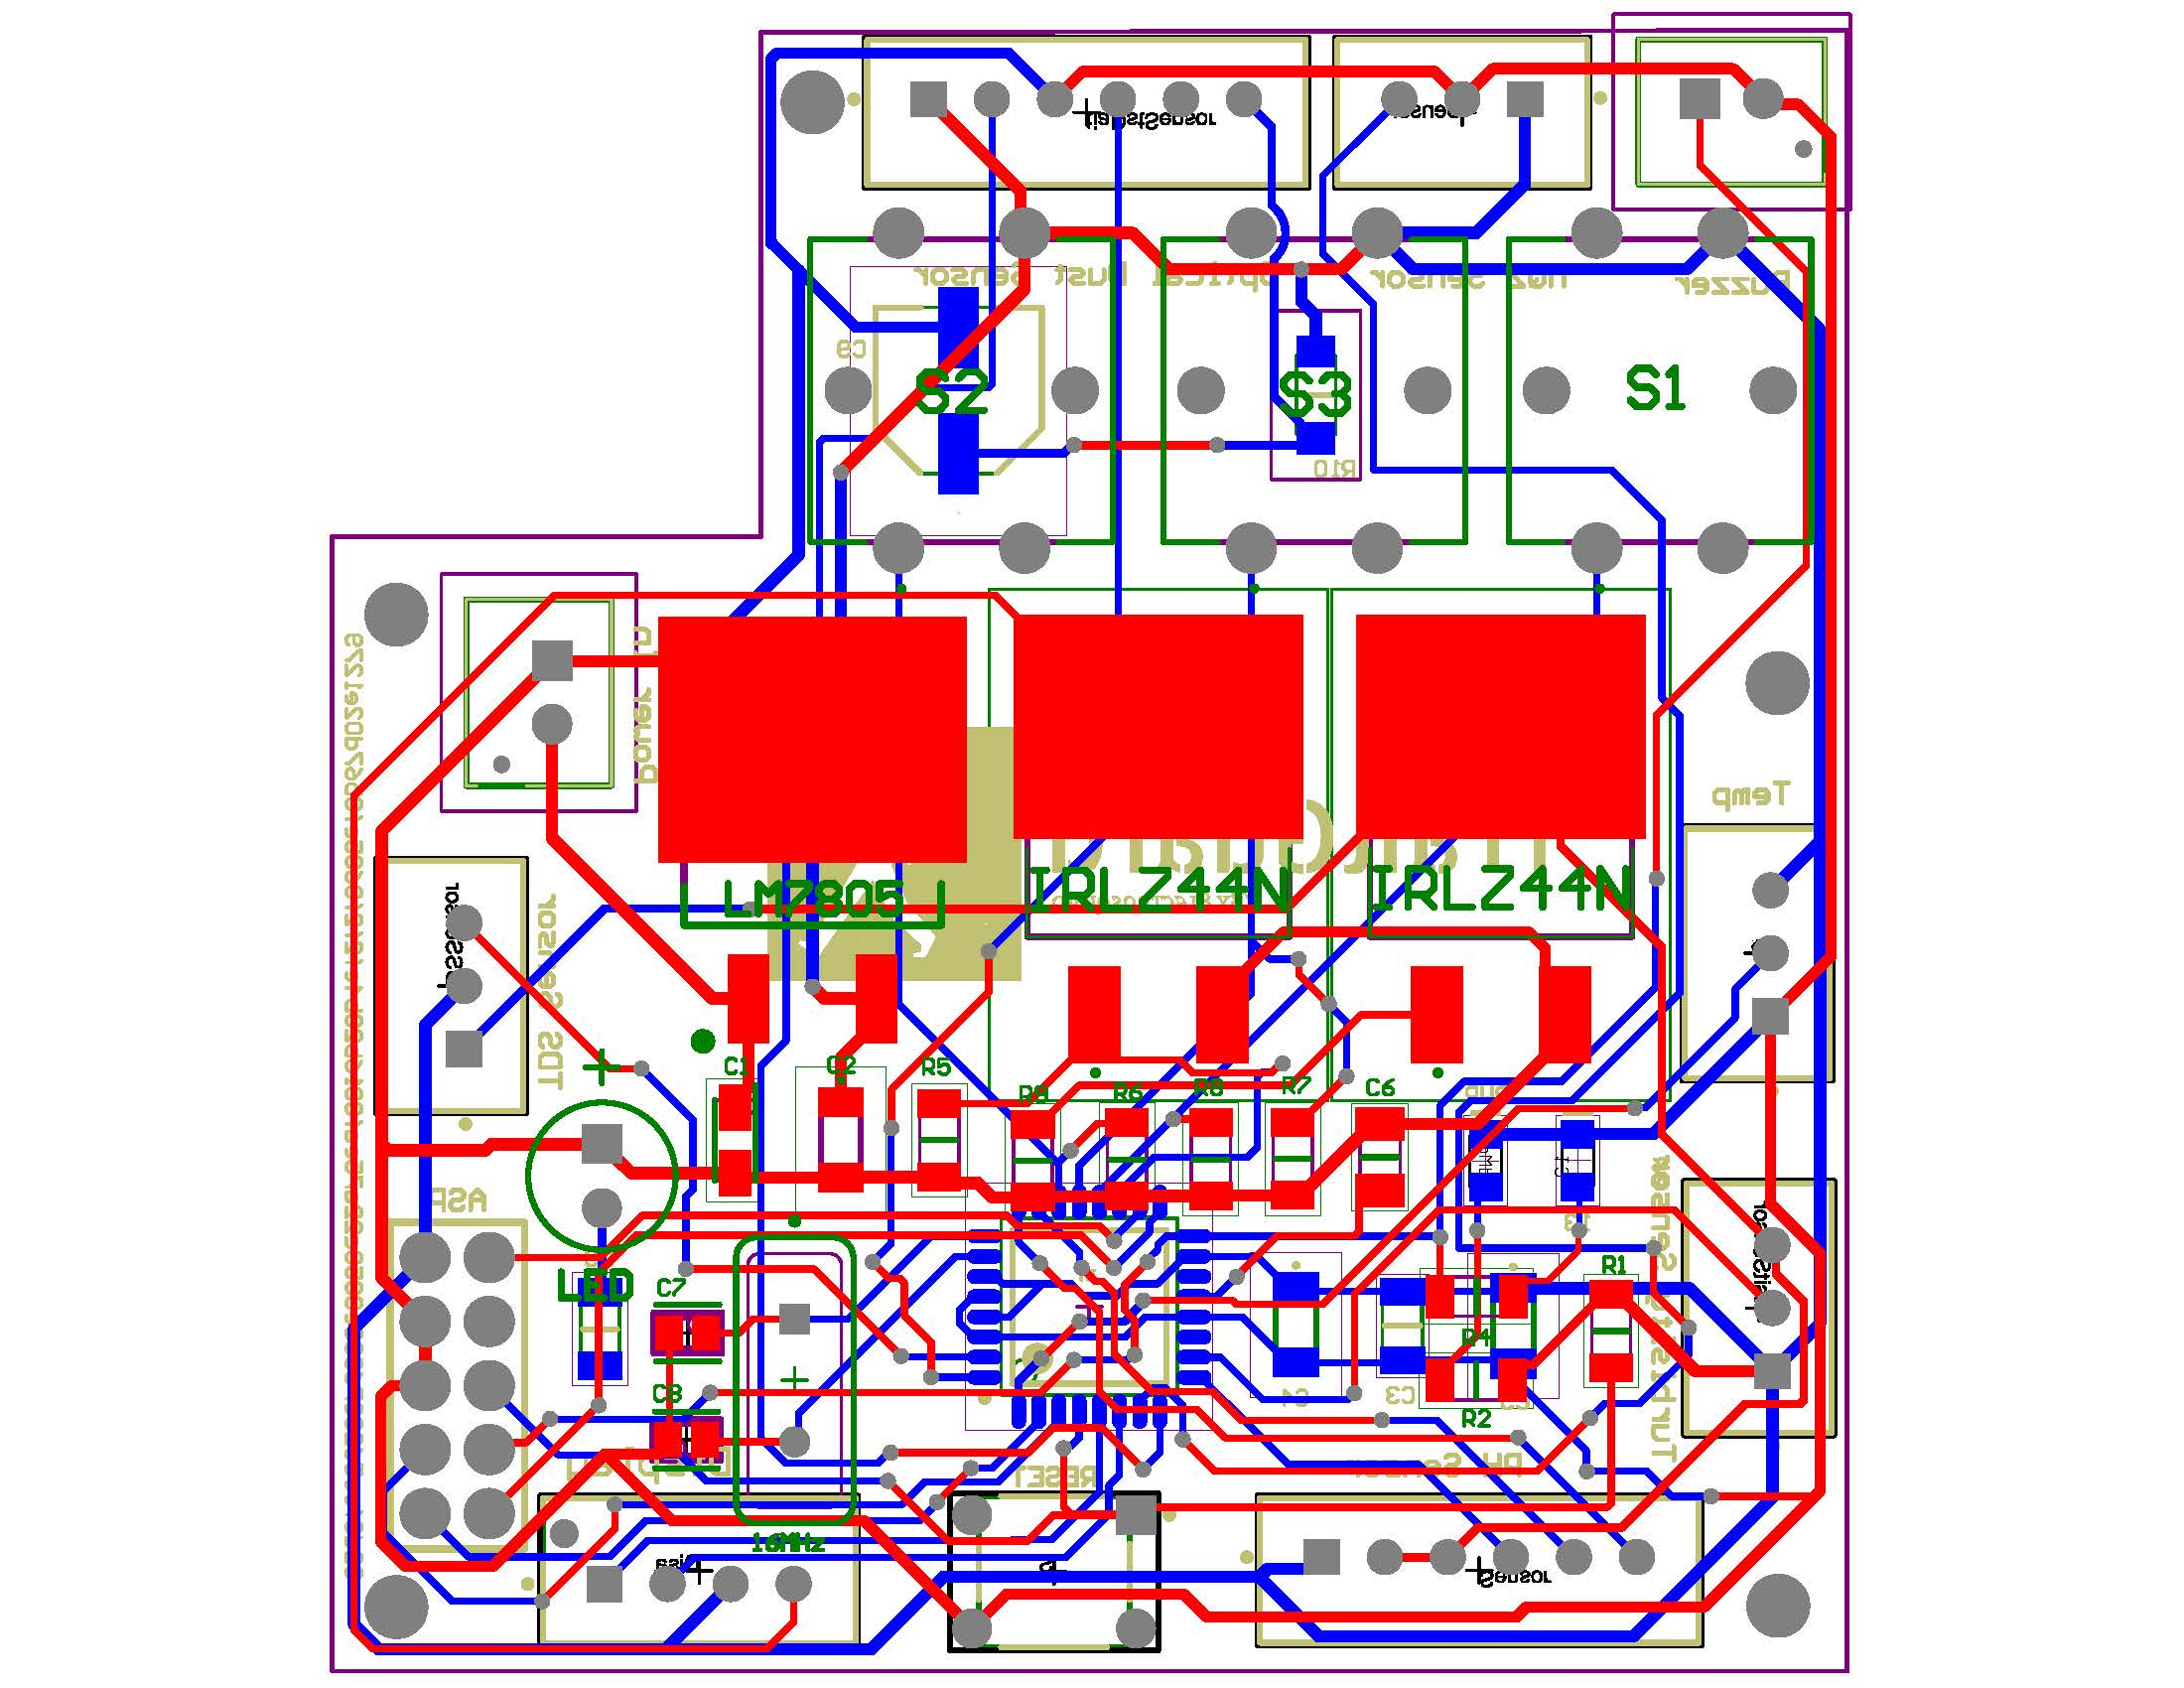
\includegraphics[width=\textwidth]{./figures/BoardStack.jpg}
        \caption{Layer Stack}
        \label{fig:image1}
    \end{subfigure}
    \hfill
    \caption{PCB Layers}
    \label{fig:threeimages}
\end{figure}

\begin{figure}[!h]
    \centering
    \begin{minipage}{0.45\textwidth}
        \centering
        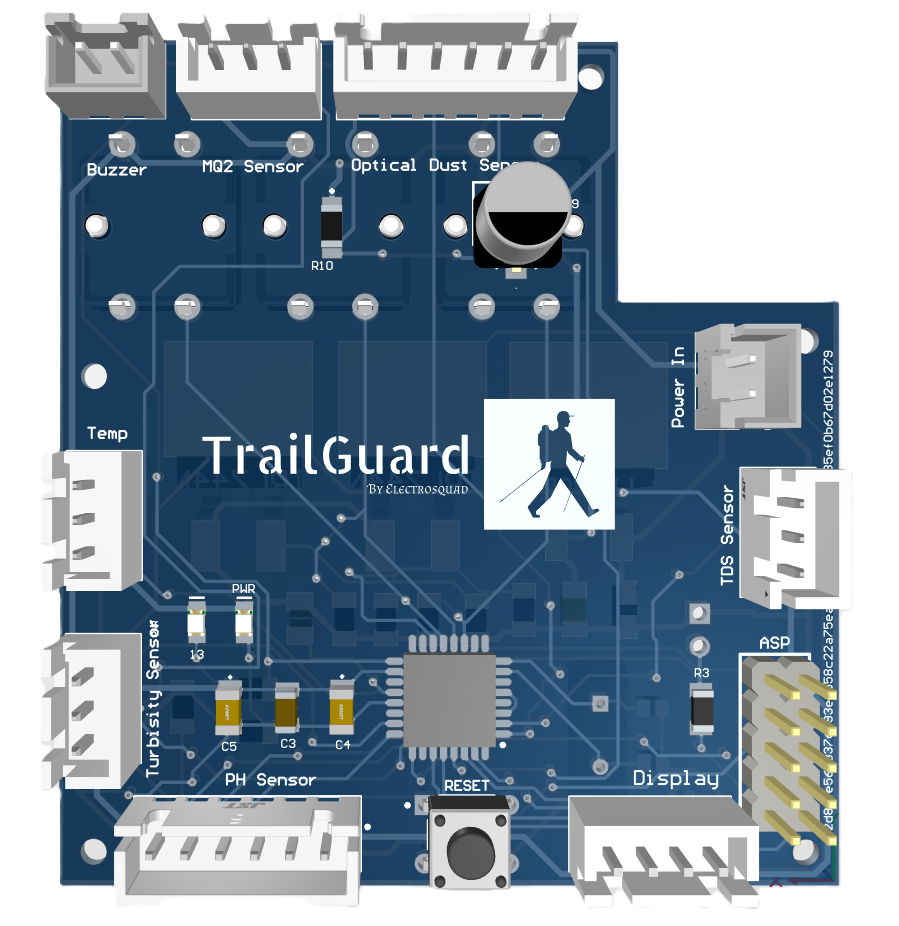
\includegraphics[width=\textwidth]{./figures/PCBDesign1.png}
        \caption{PCB top view}
    \end{minipage}\hfill
    \begin{minipage}{0.45\textwidth}
        \centering
        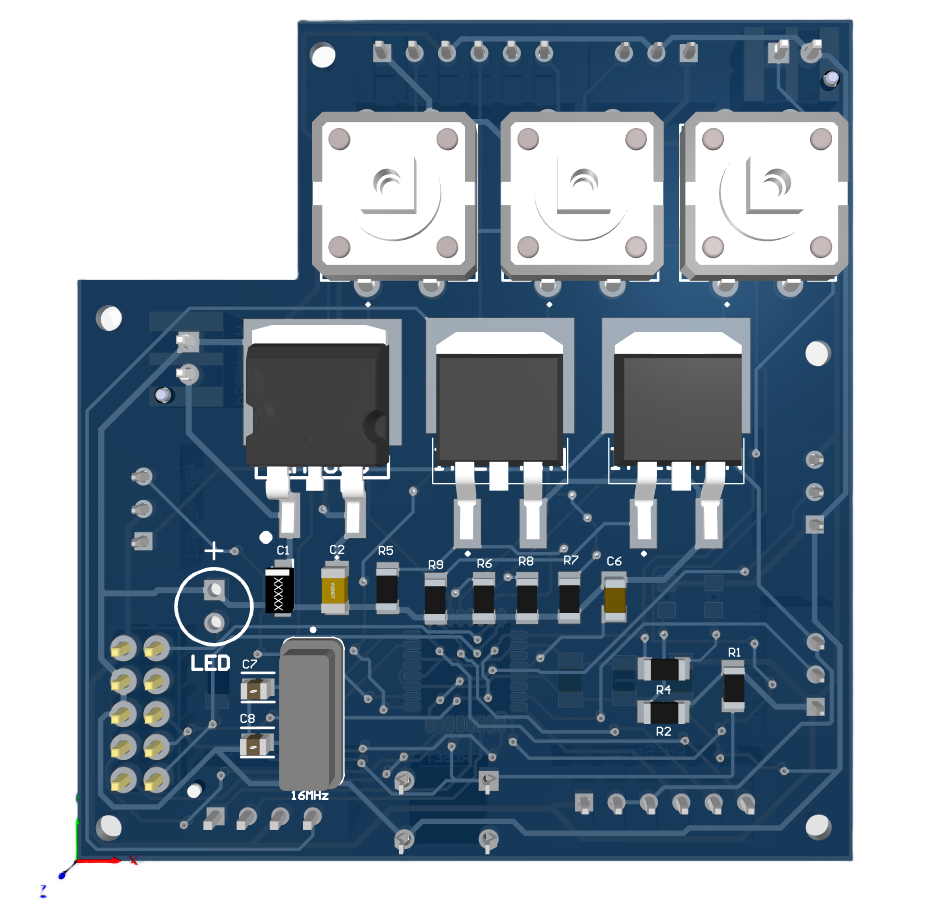
\includegraphics[width=\textwidth]{./figures/PCBDesign2.png}
        \caption{PCB bottom view}
    \end{minipage}
\end{figure}
\newpage
\subsection{PCB Schematic}
\begin{figure}[!h]
    \centering
    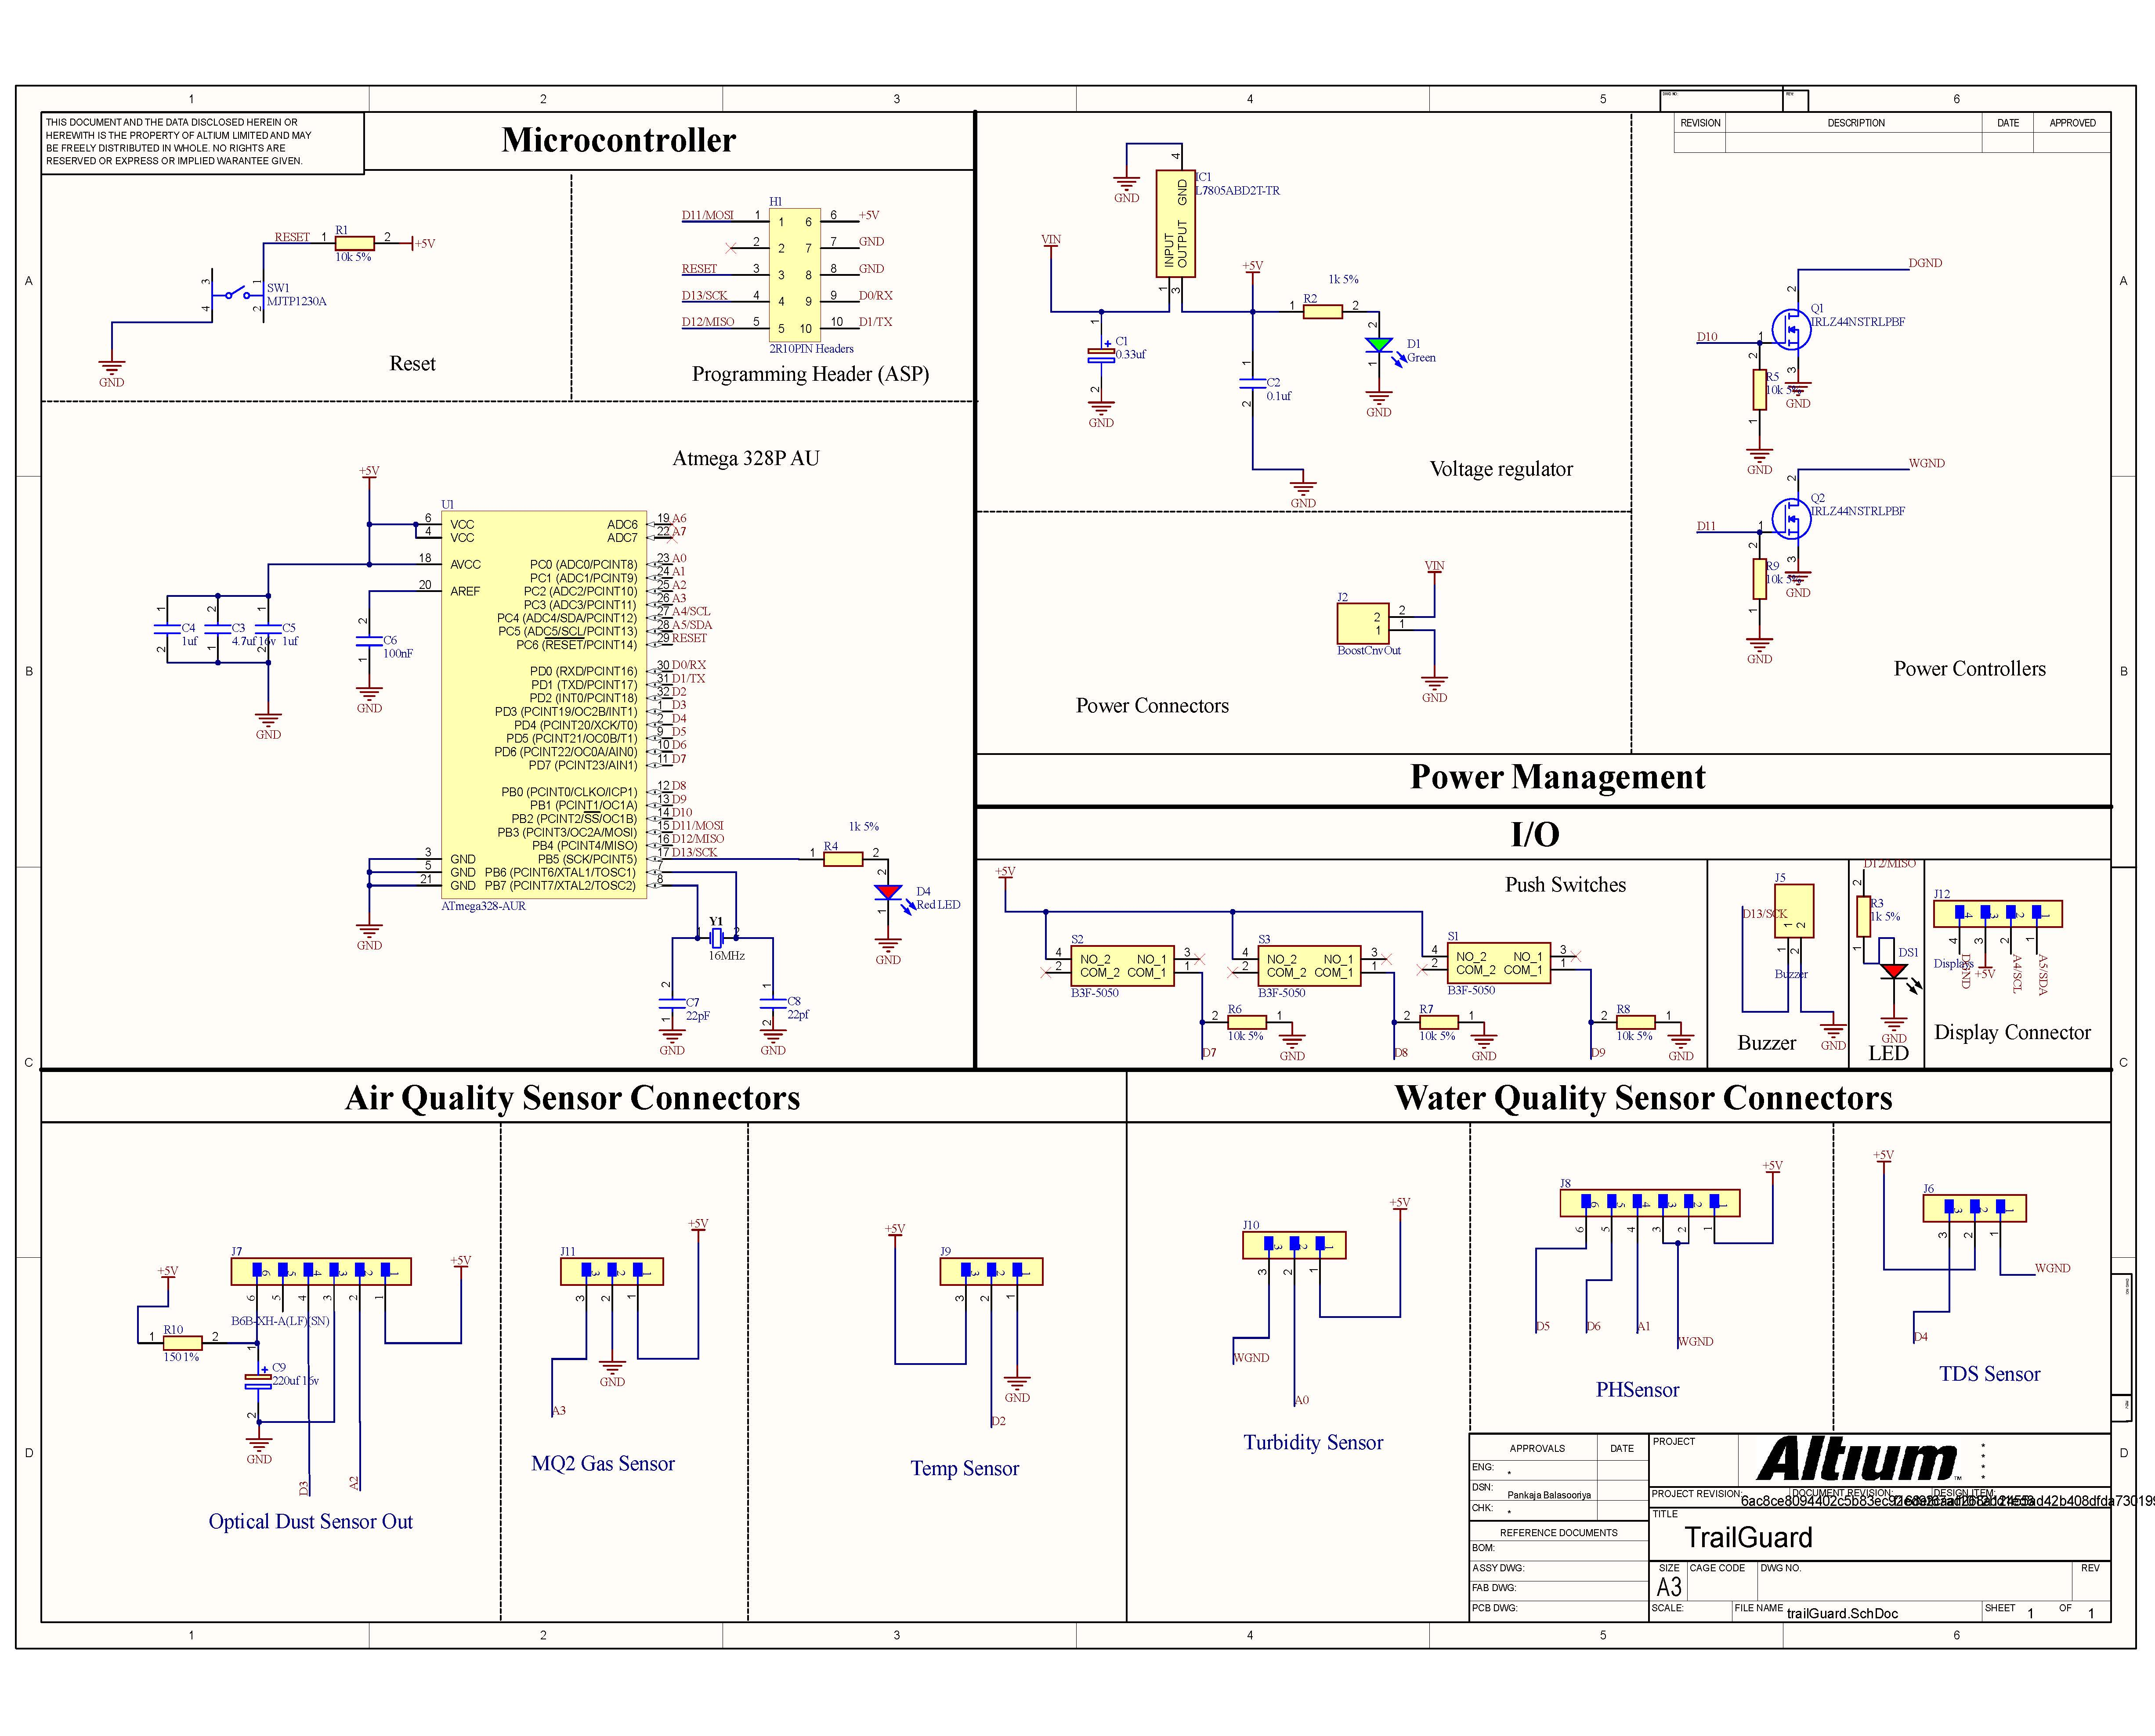
\includegraphics[scale=0.6]{./figures/PCB_schematic.jpg}
    \caption{PCB Schematic}
\end{figure}

%--------------------------------------------------------------------------
\newpage
\section{Final Product}
\begin{figure}[!h]
    \centering
    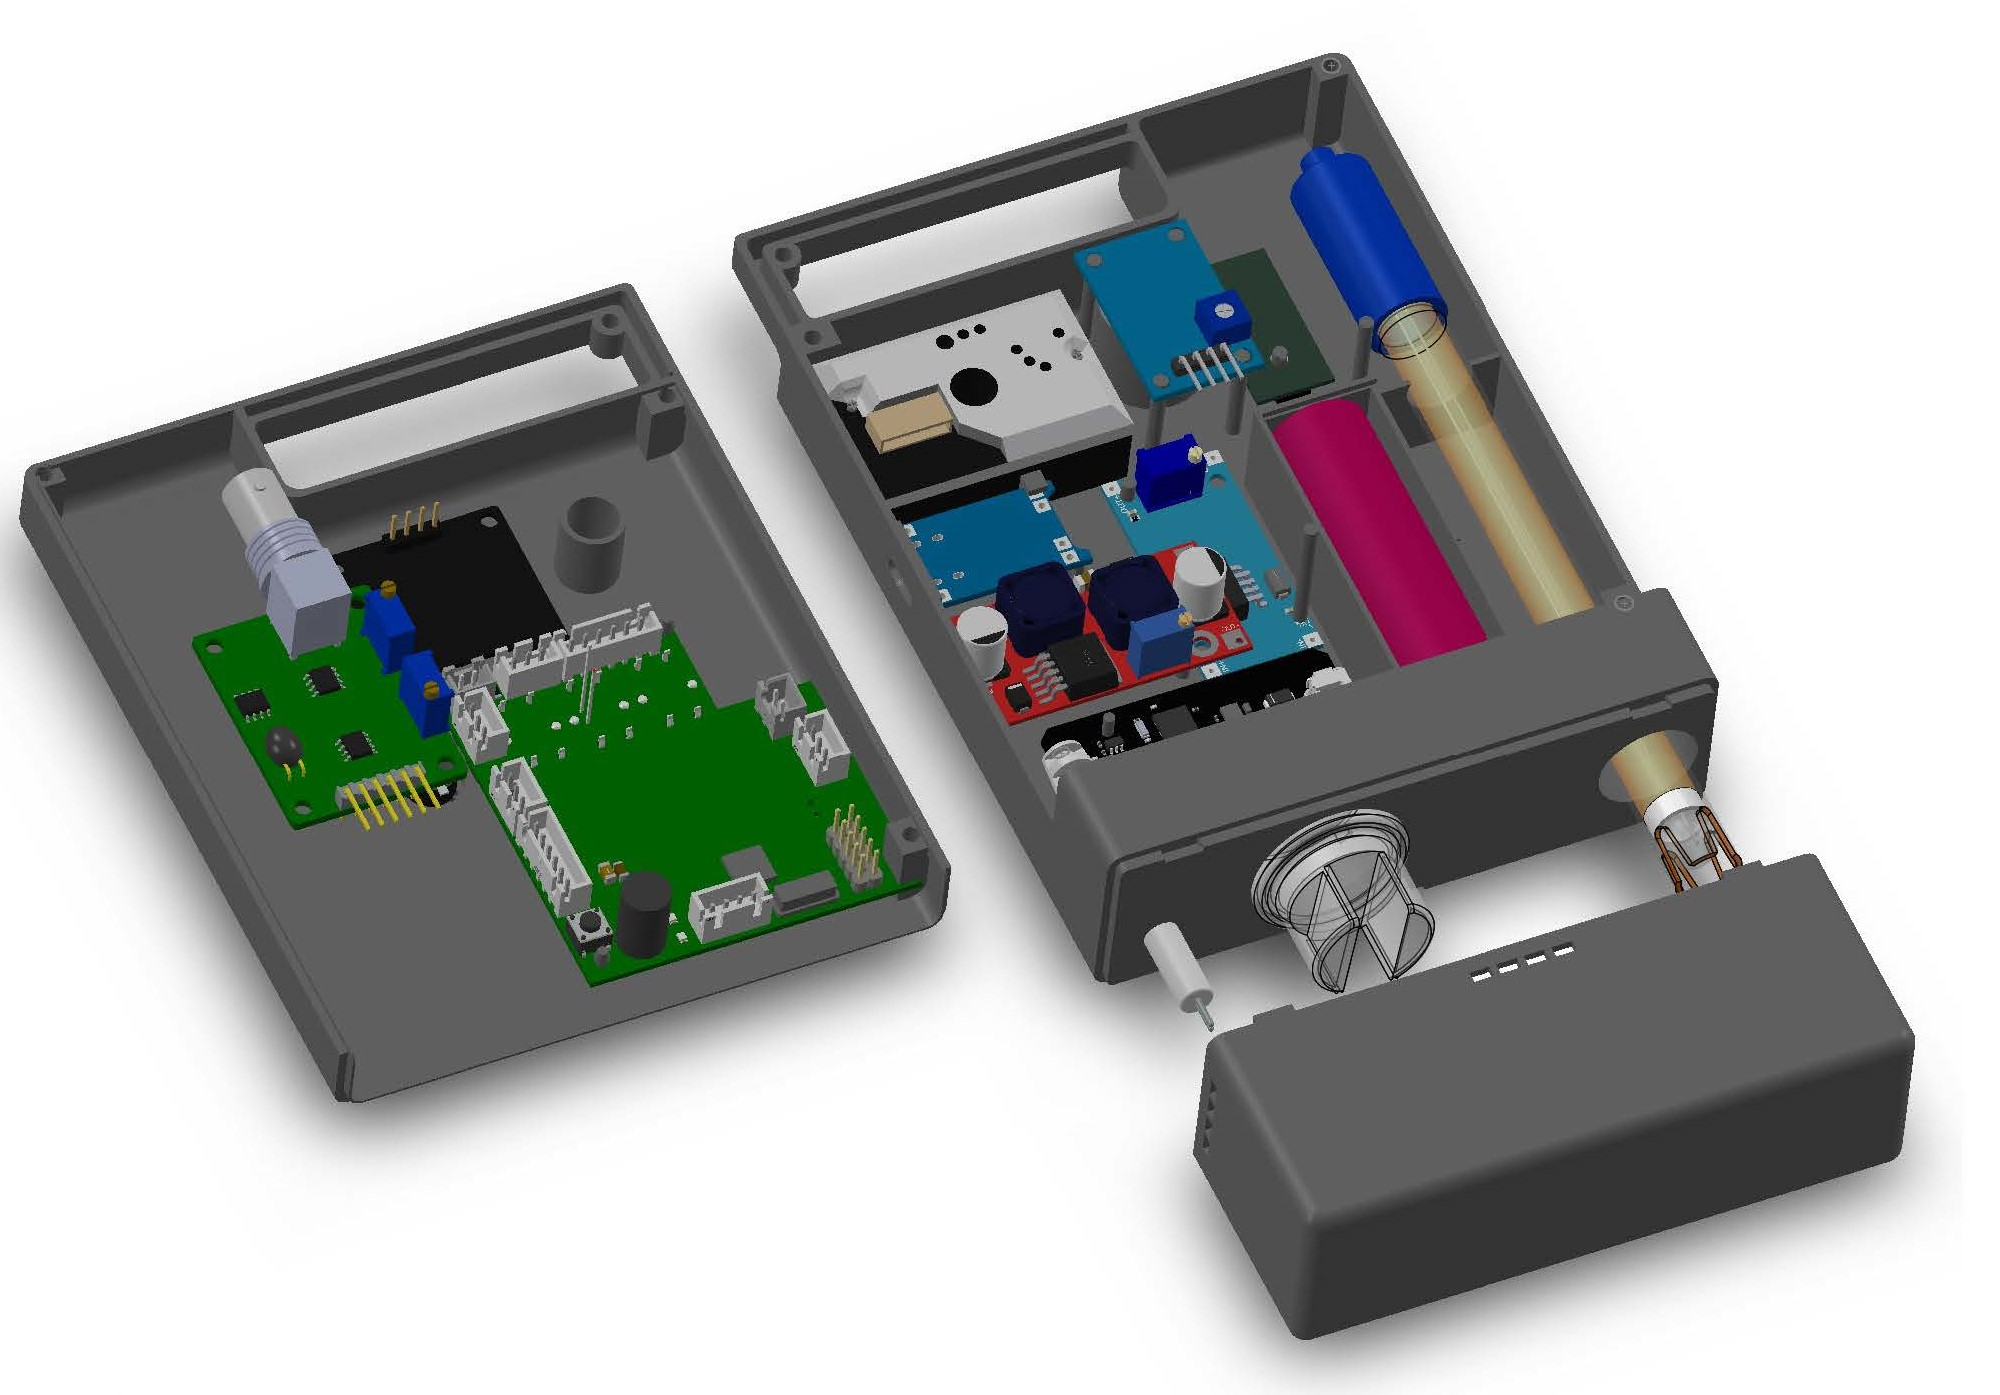
\includegraphics[scale=0.55]{./figures/finalinternal.jpg}
    \caption{Internal View of TrailGuard}
\end{figure}

\begin{figure}[!h]
    \centering
    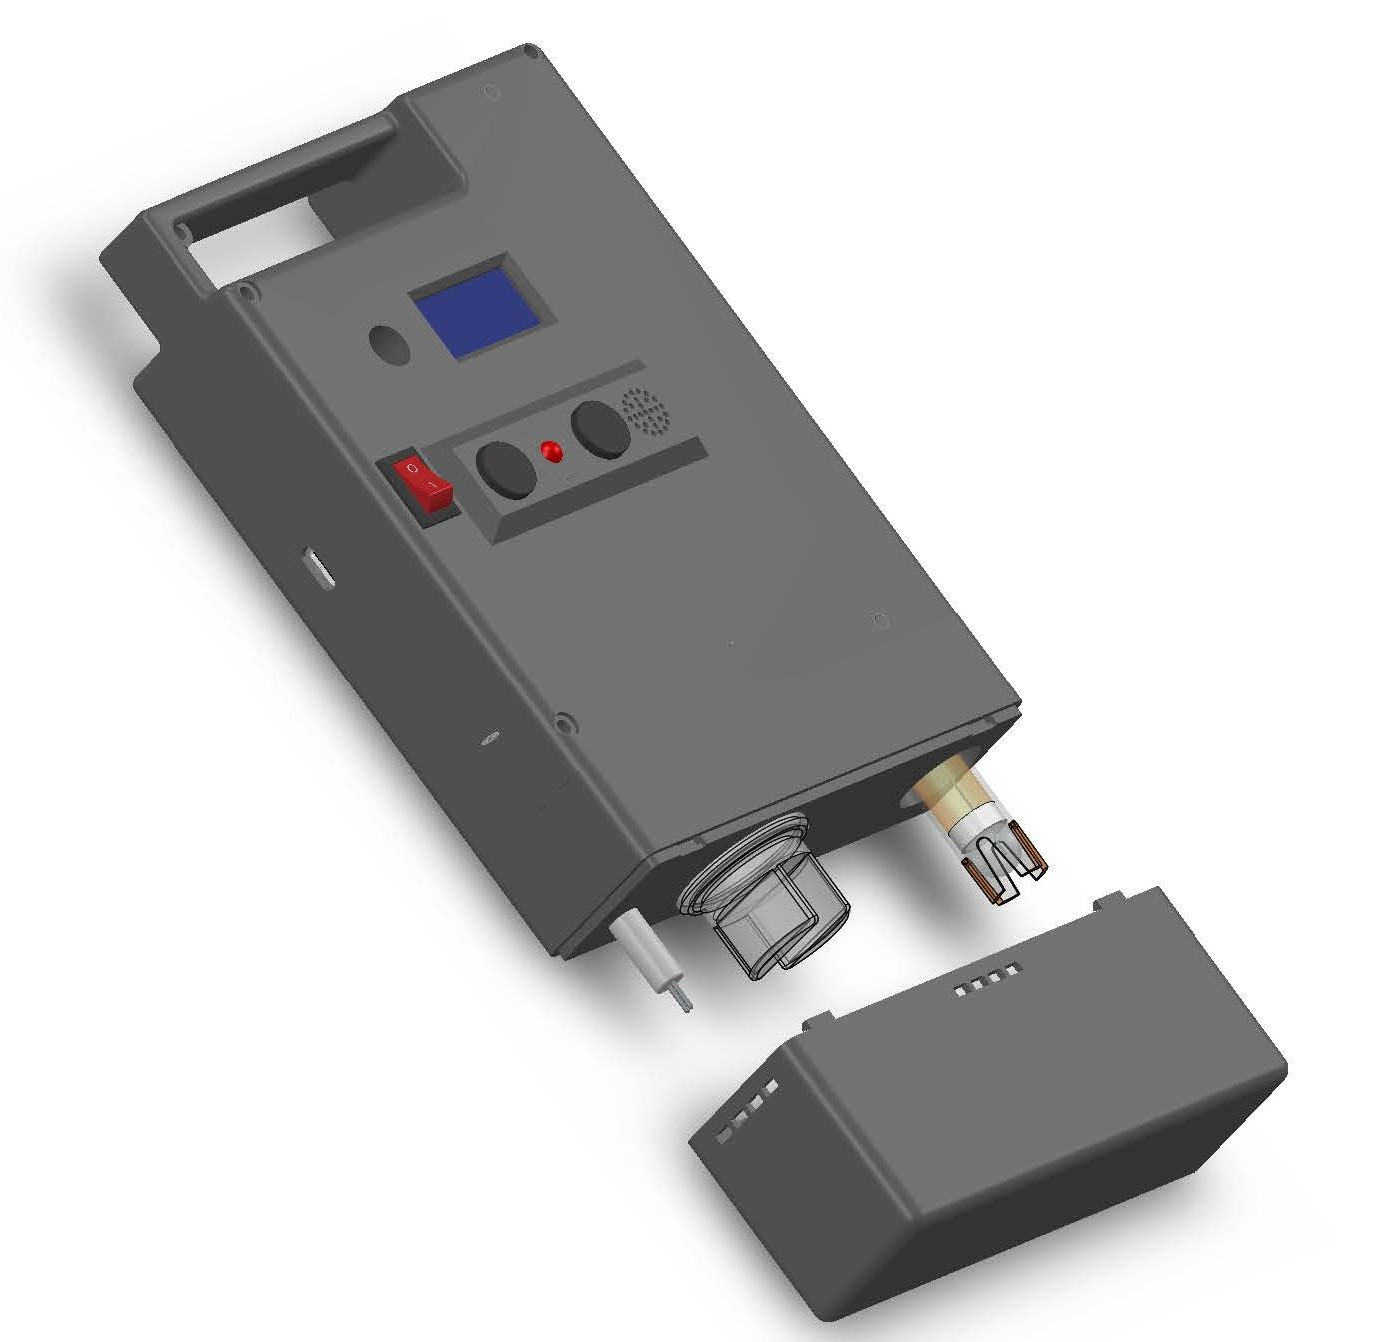
\includegraphics[scale=0.55]{./figures/FinalProduct.jpg}
    \caption{TrailGuard}
\end{figure}
%--------------------------------------------------------------------------
\newpage
\section{Marketing Strategy}
\subsection{Marketing Strategy}
\subsubsection{Target Market}
TrailGuard is primarily aimed at outdoor enthusiasts, such as hikers, campers, adventurers, and travelers who are concerned about environmental safety. Additionally, it targets residents living in areas with potential air and water quality issues, as well as educational institutions and research organizations involved in environmental monitoring. The device appeals to individuals who prioritize safety, convenience, and reliable environmental monitoring tools.

\subsubsection{Value Proposition}
TrailGuard offers a unique value proposition by combining multiple environmental monitoring functions—such as air and water quality detection, temperature, humidity measurement, and gas detection—into a single, portable device. Its compact design along with user-friendly features and easy-to-navigate interface, makes it a versatile tool for outdoor activities and daily use. Compared to existing products that only monitor either air or water quality, TrailGuard provides a comprehensive solution at a competitive price point, ensuring a high return on investment for customers.

\subsubsection{Marketing Channels}
To reach the target audience effectively, the marketing strategy will leverage multiple channels

\begin{enumerate}[a)]
	\item \textbf{Digital Marketing}
	\\ Utilize social media platforms, outdoor adventure forums, and targeted online advertising to create awareness among potential customers. A dedicated website will provide detailed product information, customer testimonials, and a platform for direct purchases.
	\item \textbf{Partnerships}
	\\ Collaborate with outdoor gear retailers and environmental organizations to promote TrailGuard. These partnerships can include co-branded marketing campaigns, product placements, and joint events.
	\item \textbf{Content Marketing}
	\\  Develop educational content such as blogs, videos, and tutorials that highlight the importance of environmental monitoring and demonstrate how TrailGuard can enhance outdoor experiences. Content will be shared across social media, YouTube, and relevant blogs.
	\item \textbf{Influencer Marketing}
	\\  Engage with influencers in the outdoor adventure and travel communities to showcase TrailGuard in real-world scenarios. Their endorsements can help build credibility and attract a wider audience.
\end{enumerate}

\subsubsection{Pricing Strategy}
TrailGuard will be priced competitively to ensure accessibility to a broad range of customers. The pricing strategy will consider the cost of production, competitor pricing, and the perceived value of the product. To attract early adopters, a limited-time discount may be offered during the product launch phase.
%--------------------------------------------------------------------------
\newpage
\section{Task Allocation}
The workload is equally distributed among the team members, with each member responsible for specific tasks based on their expertise and interests. The task allocation is as follows
\begin{table}[h]
    \centering
    \begin{tabular}{|c|c|c|}
        \hline
        \textbf{Name} & \textbf{Index Number} & \textbf{Task} \\ \hline
        Balasooriya B A P I	 & 220054N & PCB Design and Circuit Design \\ \hline
        Dewasumithra M P O & 220112R & Enclosure Design and PCB Design \\ \hline
        Dineshara M C & 220128V & Programming and Enclosure Design \\ \hline
        Diunugala C H & 220143L & Programming and Circuit Designing \\ \hline
    \end{tabular}
    \caption{Task Allocation}
    \label{tab:sample_table}
\end{table}
%--------------------------------------------------------------------------
\section{Project Budget}
\subsection{Production Cost for a single unit} 
\begin{table}[h]
    \centering
    \begin{tabular}{|c|c|c|c|}
        \hline
        \textbf{Item} & \textbf{Unit Price (LKR)} & \textbf{Quantity} & \textbf{Total Cost (LKR)} \\ \hline
        Atmega328p-AU               &   631.74 & 1 &   631.74 \\ \hline
        TS-300B Turbidity Sensor    & 2,566.86 & 1 & 2,566.86\\ \hline
        PH4502C pH Sensor           & 3,250.00 & 1 & 3,250.00\\ \hline
        DHT11 Sensor                &   230.00 & 1 &   230.00\\ \hline
        Sharp GP2Y1010AU0F Sensor   & 1,470.00 & 1 & 1,470.00\\ \hline
        MQ2 Gas Sensor              &   410.00 & 1 &   410.00\\ \hline
        Gravity TDS Sensor          & 2,350.00 & 1 & 2,350.00\\ \hline
        OLED Display (0.96")        &   600.00 & 1 &   600.00\\ \hline
        IRLZ44NSTRL MOSFET          &   150.00 & 2 &   300.00 \\ \hline
        Buttons and LEDs            &   100.00 & 1 &   100.00  \\ \hline
        Buzzer                      &    50.00 & 1 &    50.00\\ \hline
        Enclosure                   & 3,120.00 & N/A & 3,120.00\\ \hline
        Rechargeable Battery        &   760.00 & 1 &    760.00 \\ \hline
        PCB Fabrication             &   570.00 & 1 &   570.00 \\ \hline
        Miscellaneous Components    & 2,000.00 & N/A & 2,000.00  \\ \hline
        Packaging                   & 300    & 1 &     300.00 \\ \hline
        \textbf{Total Estimated Budget} & \multicolumn{3}{c|}{\textbf{18708.60}} \\ \hline
    \end{tabular}
    \caption{Project Budget for TrailGuard}
    \label{table:budget}
\end{table}
Per unit cost ccan be reduced by 20\% ordering components in bulk and further development by reducing the physcial size. Also cost can be furthur reduced by combining seperate modules and using a single probe for all readings.
\newpage
\subsection{Marketing Budget} 
Marketing budget for TrailGuard per month is estimated as follows
\begin{table}[h]
    \centering
    \begin{tabular}{|c|c|c|}
        \hline
        \textbf{Item} & \textbf{Estimated Cost (LKR)} \\ \hline
        Digital Marketing & 10,000.00 \\ \hline
        Partnerships & 5,000.00 \\ \hline
        Content Marketing & 3,000.00 \\ \hline
        Influencer Marketing & 2,000.00 \\ \hline
        \textbf{Total Estimated Budget} & \textbf{20,000.00} \\ \hline
    \end{tabular}
    \caption{Marketing Budget for TrailGuard}
    \label{table:marketing_budget}\
\end{table}
%%-----------------------------------------------------------------------

% \bibliographystyle{plain}
% bibliography{refer}

%---------------------------------------------------------------------------
\end{document}